
\section{Conclusion}
Thus far, we have built upon the definition of the multivariate Pareto described in \cite{ferreira2014}
  to establish a useful parametric representation of its dependence structure, through describing the distribution of its angular component; it being supported on the positive orthant of the unit 
  hypersphere under the $\mathcal{L}_{\infty}$ norm, $\mathcal{S}_{\infty}^{d-1}$.  We then demonstrated an
  inherent difficulty in establishing a distribution supported in this space.  To build that representation,
  we presented a distribution based on a product of independent Gammas, projected onto a supporting manifold
  $\mathcal{S}_{p}^{d-1}$, which will converge to $\mathcal{S}_{\infty}^{d-1}$ as $p\to\infty$.  We then
  established a means of model comparison on $\mathcal{S}_{\infty}^{d-1}$ through the use of a negative
  definite kernel defined in that space.

We used integrated vapor transport data--a measure of water in the atmosphere--as a motivating example for
  our model.  This data subsets California into a series of grid cells, and provides daily IVT values for
  each cell.  We used our model to develop measures of pairwise extremal dependence between grid cells, which
  could be of interest to researchers, actuaries, hydrologists and even farmers.  We additionally developed
  conditional survival functions--$\text{P}\left[Z_l > z_l\mid Z_{\not l} > z_{\not l}\right]$--which provide a more complete understanding of the dependence structure.  The reciprocal of these values provides the more well known \emph{return rates}.

We intend to leverage the information provided to us by our distribution of the angular component to build
  an efficient anomaly detection algorithm.  We have developed a preliminary analysis of two ideas for
  anomaly detection--one based on nearest neighbors, the other based on the posterior predictive loss criterion--and found them to be competitive with existing methods.  We expect development of this topic to take 3-4 months.

We finally intend to explore computational developments towards application of our model on large scale
  problems.  We find a motivating example on this topic in simulated storm-surge data, where the length of 
  a data vector can be hundreds of thousands to millions of elements long.  This topic features a pitfall in the curse of dimensionality: with current gamma or log-normal priors, model fidelity drops as the number of dimensions grows.  However, we believe a clever choice of priors for mixture components may improve model fidelity at high dimensions.  We expect development of this topic to completion to take an additional 4-5 months.
  
Finally, we expect the dissertation writing to take an additional 3-4 months beyond that.  We summarize this expected timeline in Figure~\ref{fig:timeline}.
  
\begin{figure}[hb]
  \caption{Expected timeline to defense.\label{fig:timeline}}
  \centering
  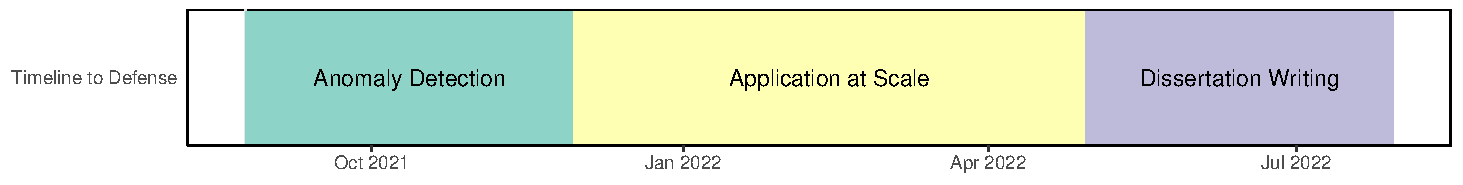
\includegraphics[width = \linewidth]{images/timeline}
\end{figure}

% EOF
